\documentclass[a4paper, 14pt]{extarticle}
\usepackage{enumitem}
\usepackage{fefutitle}
\usepackage{listings}
\usepackage{xcolor}
\usepackage{amsmath}
\usepackage{graphicx}
\usepackage[justification=centering]{caption}
\usepackage{float}

\lstdefinestyle{mystyle}{
	basicstyle={\small\ttfamily},
	keywordstyle=\color{orange},
	stringstyle=\color{green},
	basicstyle=\ttfamily\footnotesize,
	breakatwhitespace=false,         
	breaklines=true,                 
	captionpos=b,                    
	keepspaces=true,                 
	numbers=none,                    
	numbersep=5pt,                  
	showspaces=false,                
	showstringspaces=false,
	showtabs=false,                  
	tabsize=2,
	aboveskip=3mm,
	belowskip=3mm,
}
\lstset{style=mystyle}

\begin{document}
	\fefutitle{2}
	\pagebreak	

	\section{Определение цели}
		В данной лабораторной работе нужно создать математическую модель движения материальной точки во вращающейся системе координат. При движении относительно вращающейся системы координат на точку действует сила Кориолиса. Добавление силы Кориолиса к действующим на материальную точку физическим силам позволяет учесть влияние вращения системы отсчёта на такое движение. Названа по имени французского учёного Гаспара-Гюстава де Кориолиса, впервые описавшего её в статье, опубликованной в 1835 году.

	\section{Создание математической модели}
		\[ m\dfrac{d\vec{\upsilon}}{dt} = F_k\]
		\[ \vec{F_k} = 2\cdot\vec{\Omega}\times\vec{V} \]
		
		\[\begin{cases}
			m\dfrac{du}{dt} = 2\cdot\upsilon m,\\
			m\dfrac{d\upsilon}{dt} = 2\cdot u m,\\
			\dfrac{dx}{dt} = u,\\
			\dfrac{dy}{dt} = \upsilon;\\
		\end{cases}\]
		
		\[\begin{cases}
			\dfrac{du}{dt} = 2\cdot\upsilon,\\
			\dfrac{d\upsilon}{dt} = 2\cdot u,\\
			\dfrac{dx}{dt} = u,\\
			\dfrac{dy}{dt} = \upsilon.\\
		\end{cases}\]
	
	\section{Реализация модели}
		Модель была реализована в Mathcad.
		\[
		V_1 = \begin{bmatrix}x_0=5,\\y_0=3,\\u_0=5,\\\upsilon_0=5,\\\omega=1.\end{bmatrix}
		V_2 = \begin{bmatrix}x_0=5,\\y_0=3,\\u_0=5,\\\upsilon_0=5,\\\omega=1.\end{bmatrix}
		V_3 = \begin{bmatrix}x_0=5,\\y_0=3,\\u_0=5,\\\upsilon_0=5,\\\omega=1.5.\end{bmatrix}
		V_4 = \begin{bmatrix}x_0=5,\\y_0=3,\\u_0=5,\\\upsilon_0=5,\\\omega=0.5.\end{bmatrix}
		\]
		\begin{figure}[H]
			\centering
			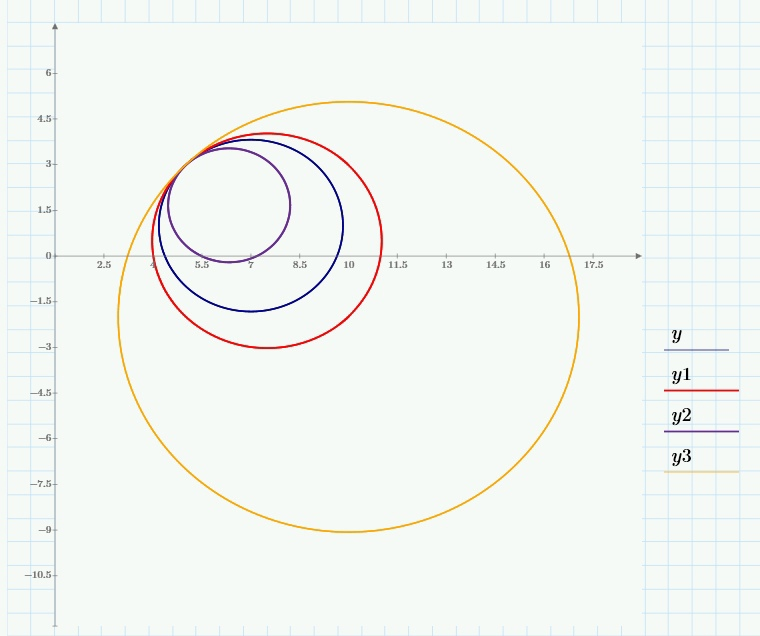
\includegraphics[width = \linewidth]{1.jpg}
			\caption{Траектории движения}
		\end{figure}
		\begin{figure}[H]
			\centering
			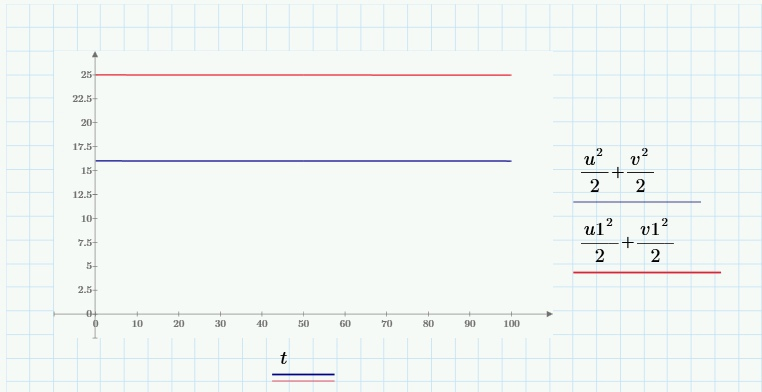
\includegraphics[width = \linewidth]{2.jpg}
			\caption{Графики зависимости $u^2+\upsilon^2$ от $t$}
		\end{figure}
		\begin{figure}[H]
			\centering
			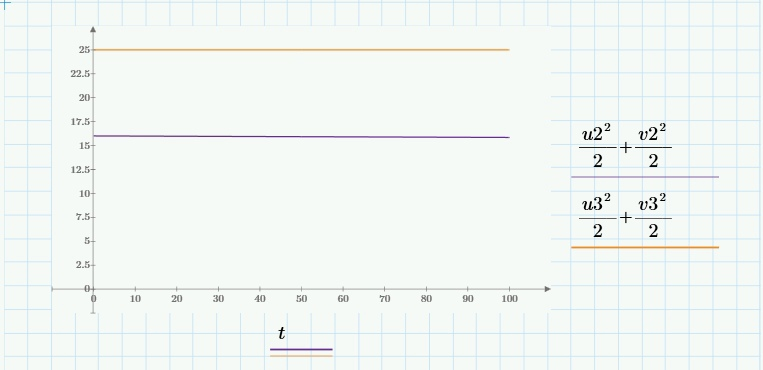
\includegraphics[width = \linewidth]{3.jpg}
			\caption{Графики зависимости $u^2+\upsilon^2$ от $t$}
		\end{figure}
		
	\section{Вывод}

		
\end{document}	